\documentclass{if-beamer}
\usepackage{ragged2e}
\usepackage{mathtools}
\usepackage{multirow}
\usepackage{setspace}
\usepackage{gensymb}
\usepackage{amsmath, amssymb}
\usepackage{caption}
%\usepackage{multirow}
%\usepackage{multicolumn}
%\usepackage{subcaption}
%\doublespacing
\singlespacing
\usepackage{csvsimple}
\usepackage{amsmath}
\usepackage{multicol}
%\usepackage{enumerate}
\usepackage{amssymb}
%\usepackage{graphicx}
\usepackage{newfloat}
%\usepackage{syntax}
\usepackage{listings}

\usepackage{color}
\usepackage{tikz}
\usetikzlibrary{shapes,arrows}



%\usepackage{graphicx}
%\usepackage{amssymb}
%\usepackage{relsize}
%\usepackage[cmex10]{amsmath}
%\usepackage{mathtools}
%\usepackage{amsthm}
%\interdisplaylinepenalty=2500
%\savesymbol{iint}
%\usepackage{txfonts}
%\restoresymbol{TXF}{iint}
%\usepackage{wasysym}
\usepackage{amsthm}
\usepackage{mathrsfs}
\usepackage{txfonts}
\usepackage{stfloats}
\usepackage{cite}
\usepackage{cases}
\usepackage{mathtools}
\usepackage{caption}
\usepackage{enumerate}	
\usepackage{enumitem}
\usepackage{amsmath}
%\usepackage{xtab}
\usepackage{longtable}
\usepackage{multirow}
%\usepackage{algorithm}
%\usepackage{algpseudocode}
\usepackage{enumitem}
\usepackage{mathtools}
\usepackage{hyperref}


% --------------------------------------------------- %
%                  Presentation info	              %
% --------------------------------------------------- %
\title[Paper II Q8]{The Maths involved in Voice Recognition}
\subtitle{An ML Assignment}
\author{Nikhil P}
\institute[IITH]{
  Indian Institute of technology \\
  Hyderabad
}
\date{\today}
\logo{

\includegraphics[scale=0.15]{index.png}
}
\subject{Presentation subject} % metadata

\graphicspath{{figuras/}}
% --------------------------------------------------- %
%                    Title + Schedule                 %
% --------------------------------------------------- %

\begin{document}

\begin{frame}
  \titlepage
\end{frame}


% --------------------------------------------------- %
%                      Presentation                   %
% --------------------------------------------------- %
\begin{frame}{Table of contents}
  \tableofcontents
\end{frame}




\subsection{Zero Padding}
\begin{frame}{Zero Padding}
Zero padding consists of extending a signal (or spectrum) with zeros. It maps a length $ N$ signal to a length $ M>N$ signal, but $ N$ need not divide $ M$. This is used to multiply the original 80 files to 2000 in number.
\begin{figure}
\centering
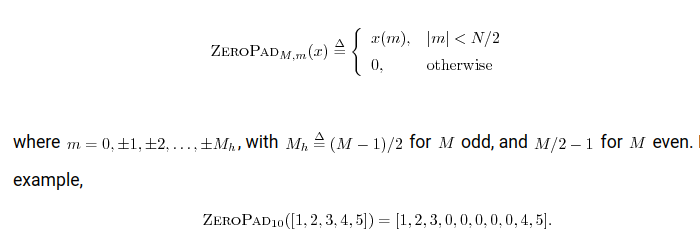
\includegraphics[width=0.8\columnwidth]{Img1.png}
%\caption{Circle $C$ and .}
\label{fig:FinalPres1}
\end{figure}
\textit{Code:
 \href{https://github.com/NikhilPraveen/College/tree/master/AIandML/ToyCar/250files.py}{250files.py}}

\end{frame}

\subsection{MFCC}
\begin{frame}{MFCC}
The features of the given audio sample is detected by first changing the clip to a matrix and using the MFCC function from Librosa. This gives a matrix of dimension 49x39 i.e the file is broken down to 49 time-steps, with each step having 39 features.
 
\end{frame}

\subsection{Recurrring Neural Network}
\begin{frame}{Recurrent Neural Network}
Recurrent Neural Network(RNN) are a type of Neural Network where the output from previous step are fed as input to the current step. \\ \text{ }
\\In traditional neural networks, all the inputs and outputs are independent of each other, but in cases like when it is required to predict the next word of a sentence, the previous words are required and hence there is a need to remember the previous words. \\ \text{}
\\Thus RNN came into existence, which solved this issue with the help of a Hidden Layer.\\  \text{}
\\The main and most important feature of RNN is Hidden state, which remembers some information about a sequence.
\end{frame}
\begin{frame}
In a normal Nueral Network, each hidden layer will have its own set of weights and biases, let’s say, for hidden layer 1 the weights and biases are (w1, b1), (w2, b2) for second hidden layer and (w3, b3) for third hidden layer. \\This means that each of these layers are independent of each other, i.e. they do not memorize the previous outputs.\\ \text{}



Now, RNN does the following 
\begin{list}
    
    \item  $\textbf(A)$ RNN converts the independent activations into dependent activations by providing the same weights and biases to all the layers, thus reducing the complexity of increasing parameters and memorizing each previous outputs by giving each output as input to the next hidden layer.
    \item $\textbf(B)$ Hence these three layers can be joined together such that the weights and bias of all the hidden layers is the same, into a single recurrent layer.
\begin{figure}
\centering
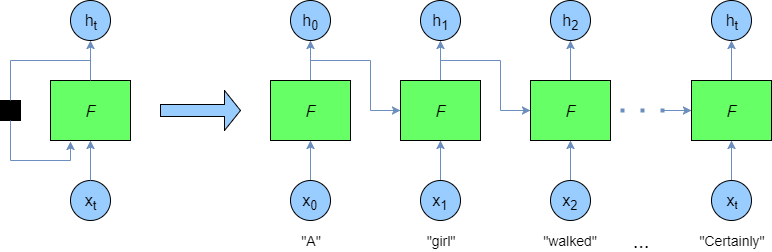
\includegraphics[width=0.8\columnwidth]{RNN.png}
%\caption{Circle $C$ and .}
\label{fig:FinalPres1}
\end{figure}
    
\end{list}
\end{frame}

\begin{frame}{LSTM}
Here,we use a variant of RNN,called LSTM ( Long Short Term Memory), in which a gate called forget gate is implemented, that makes the output from non-related nodes insignificant, i.e the overall weight given depends only on the relevant nodes.
\begin{figure}
\centering
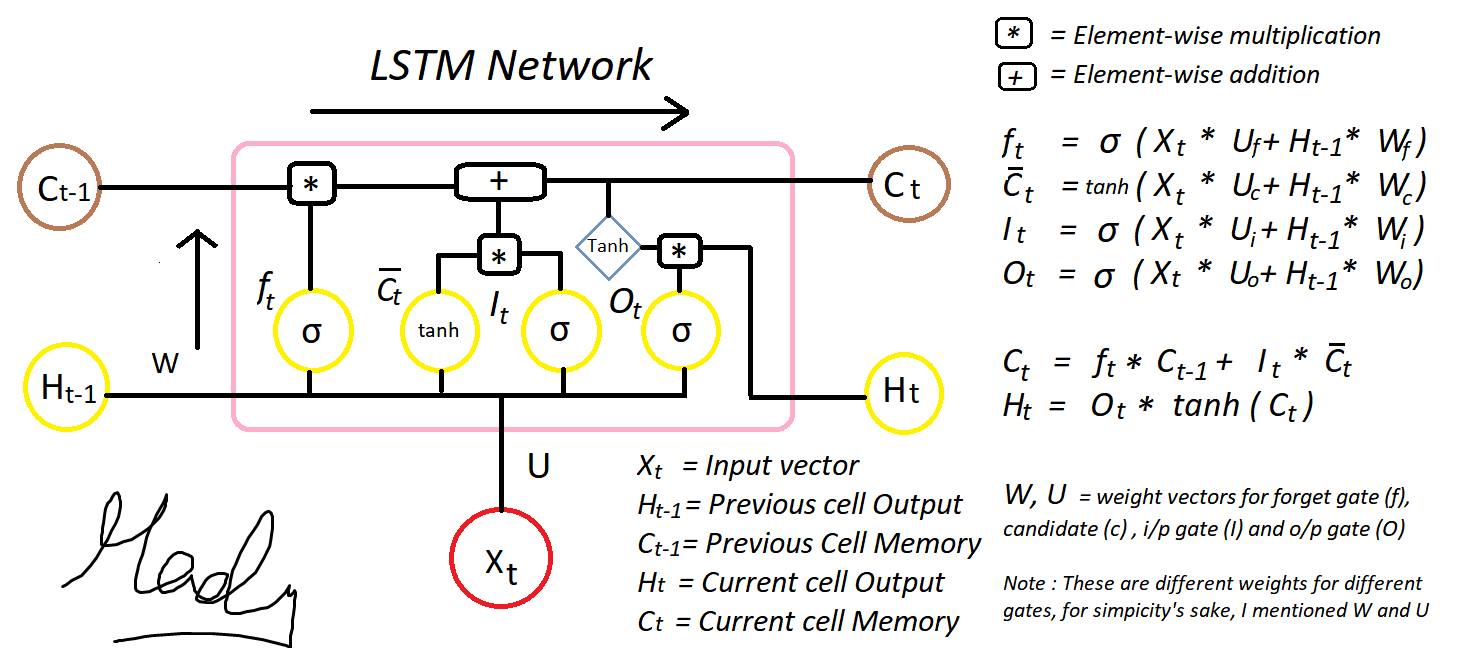
\includegraphics[width=0.8\columnwidth]{LSTM.png}
%\caption{Circle $C$ and .}
\label{fig:FinalPres1}
\end{figure}
\end{frame}
\subsection{Loss Function}
\begin{frame}{Loss Function}

The output of the LSTM is compared to the required output during training by the use of a loss function called Categorical Cross Entropy given by

\begin{figure}
\centering
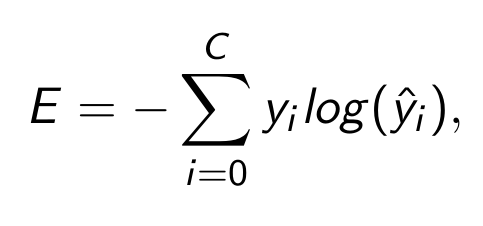
\includegraphics[width=0.3\columnwidth]{CCE.png}
%\caption{Circle $C$ and .}
\label{fig:FinalPres1}
\end{figure}
\end{frame}
,where C is the total no. of Classes




















\end{document}
